\documentclass[10pt, a4paper]{article}

\usepackage{ctex}
\usepackage{xeCJK}
\usepackage{caption}
\usepackage{geometry}
\geometry{
    left = 0.6in,
    right = 0.6in,
    top = 0.8in,
    bottom = 1.0in
}
\usepackage{amssymb}
\usepackage{amsbsy}
\usepackage{amsmath}
\usepackage{xcolor}
\usepackage{mathrsfs}
\usepackage{graphicx}
\usepackage{pifont}
\usepackage{tasks}
\settasks{
    label = \Alph*. ,
    label-width = 16pt
}
\pagestyle{empty}

\newcommand{\Title}[3]{
    \begin{center}
        \Large \textbf{中国电子学会 #1~年~#2~月 Scratch~#3级考试}
    \end{center}
}
\newcommand{\TimeAndName}[1]{
    \begin{center}
        考试时间:~#1~ 分钟 \qquad\qquad\qquad\qquad 姓名:\underline{\quad\quad\quad\quad}
    \end{center}
}

\begin{document}
    \Title{2021}{3}{二} % 标题
    \TimeAndName{60} % 考试时间及姓名

    % 单选题
    \vspace{2mm}
    {\noindent\textbf{第一部分、单选题(共 25 题,每题 2 分,共50分.)}}
    \begin{enumerate}
        % 1
        \item  小猫在沙漠中旅行好不容易找到了一杯水,初始位置如下图所示,下面哪个程序可以帮助它成功喝到水?(\qquad)
        \begin{tasks}(4)
            \task 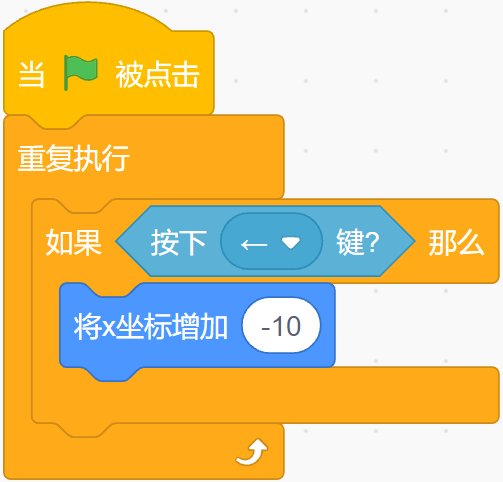
\includegraphics[width=.15\textwidth]{1a.png}
            \task 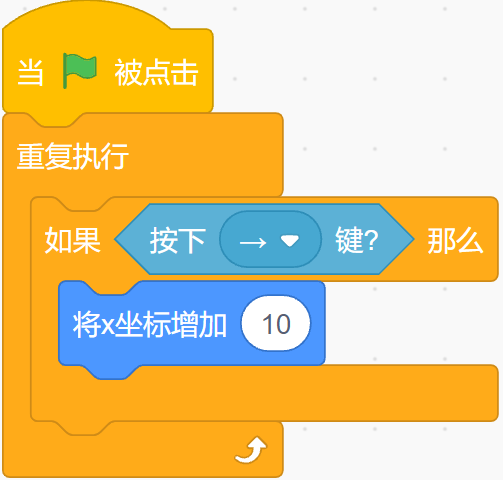
\includegraphics[width=.15\textwidth]{1b.png}
            \task 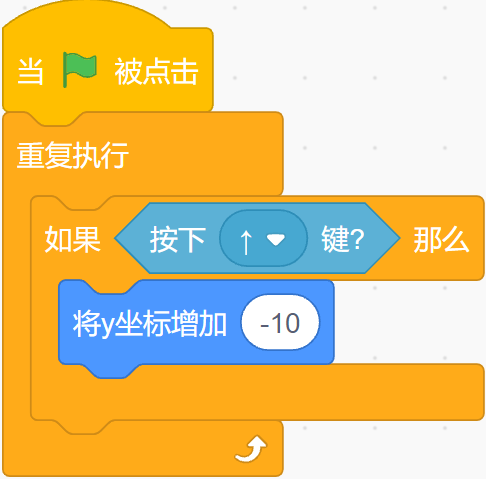
\includegraphics[width=.15\textwidth]{1c.png}
            \task 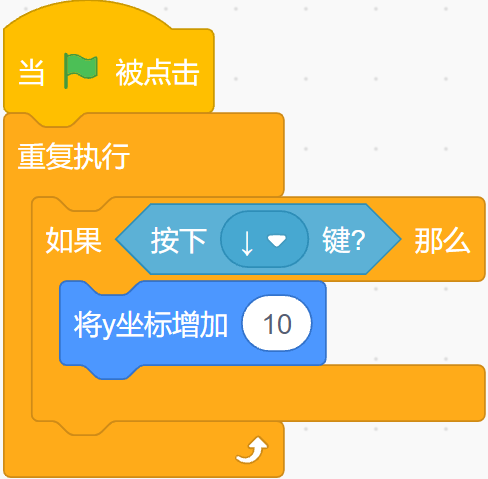
\includegraphics[width=.15\textwidth]{1d.png}
        \end{tasks}

        \begin{figure}[htbp]
            \centering
            \begin{minipage}[t]{.18\textwidth}
                \centering
                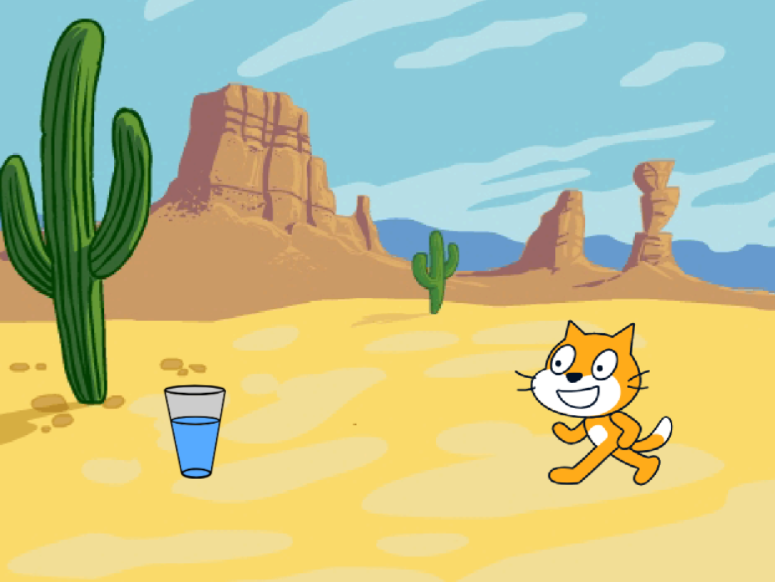
\includegraphics[width=\textwidth]{1.png}
                \caption*{第1题}
            \end{minipage}
            \begin{minipage}[t]{.15\textwidth}
                \centering
                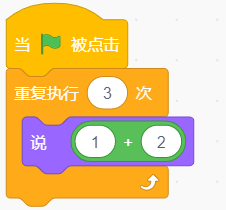
\includegraphics[width=\textwidth]{2.png}
                \caption*{第2题}
            \end{minipage}
            \begin{minipage}[t]{.6\textwidth}
                \begin{minipage}[t]{.32\textwidth}
                    \centering
                    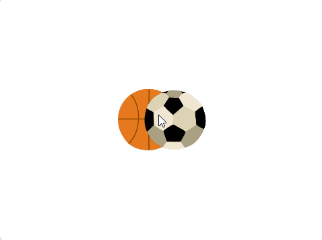
\includegraphics[width=\textwidth]{4-1.png}
                \end{minipage}
                \begin{minipage}[t]{.32\textwidth}
                    \centering
                    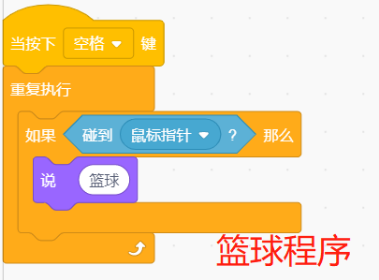
\includegraphics[width=\textwidth]{4-2.png}
                \end{minipage}
                \begin{minipage}[t]{.32\textwidth}
                    \centering
                    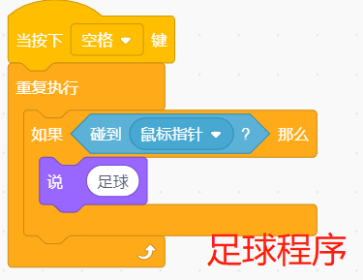
\includegraphics[width=\textwidth]{4-3.png}
                \end{minipage}
                \caption*{第4题}
            \end{minipage}
        \end{figure}

        % 2
        \item 执行上面程序,角色说的内容是?(\qquad)
        \begin{tasks}(4)
            \task 333
            \task 121212
            \task 3
            \task 12
        \end{tasks}

        % 3
        \item 执行如图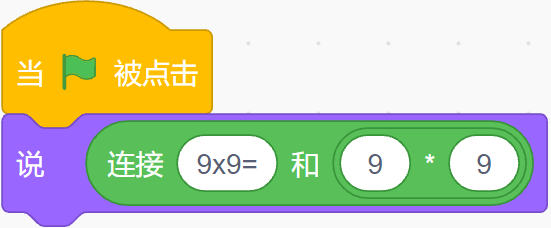
\includegraphics[width=.2\textwidth]{3.png}程序,角色说的内容是?(\qquad)
        \begin{tasks}(4)
            \task $9 \times 9 = 81$
            \task $9 \times 9 = 8*1$
            \task $9*9 = 81$
            \task $9*9 = 8*1$
        \end{tasks}

        % 4
        \item 舞台上篮球和足球角色如下图位置摆放,把鼠标移到角色重叠处后按下空格键,下面哪个选项是正确的?(\qquad)
        \begin{tasks}(2)
            \task 只显示“篮球”
            \task 只显示“足球”
            \task 同时显示“篮球”“足球”
            \task 不显示任何信息
        \end{tasks}

        % 5
        \item 下列哪个选项,可以将画笔的粗细值调整为30?(\qquad)
        \begin{tasks}(4)
            \task 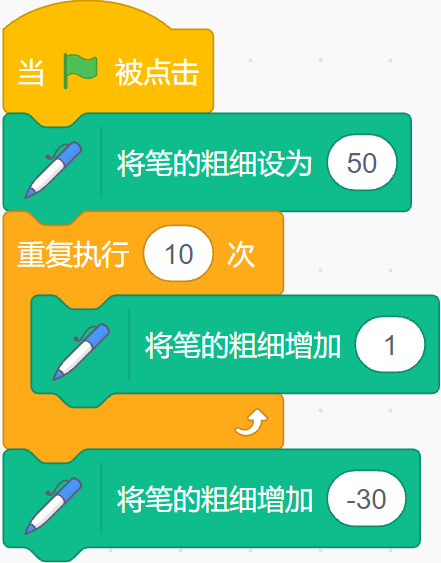
\includegraphics[width=.15\textwidth]{5a.png}
            \task 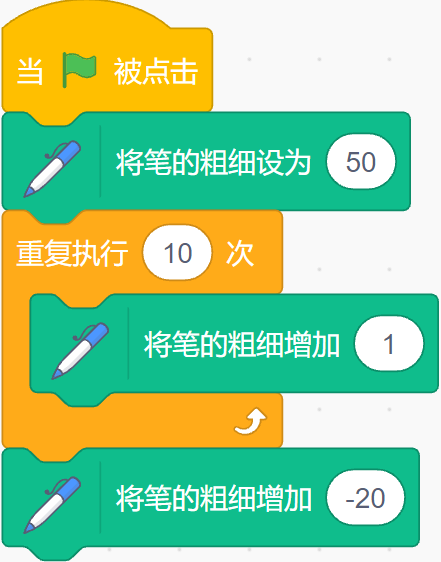
\includegraphics[width=.15\textwidth]{5b.png}
            \task 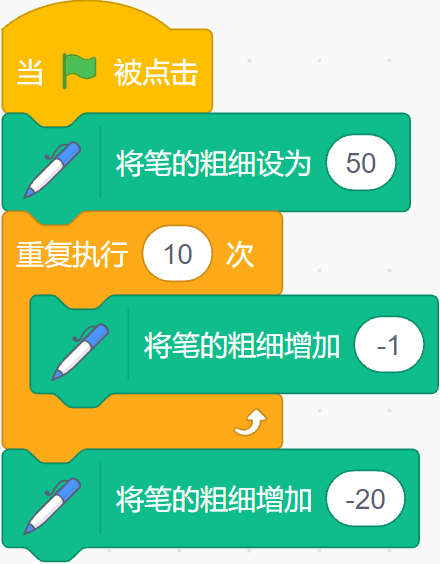
\includegraphics[width=.15\textwidth]{5c.png}
            \task 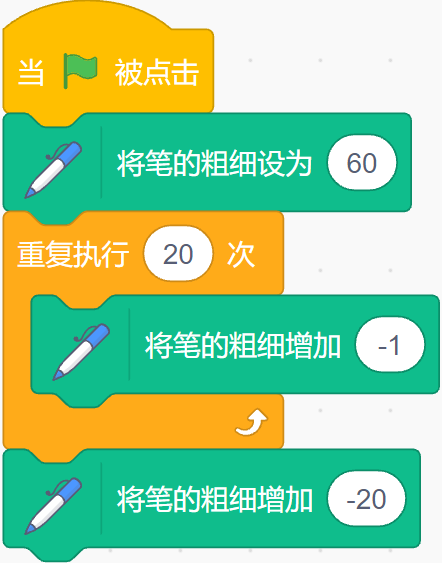
\includegraphics[width=.15\textwidth]{5d.png}
        \end{tasks}

        % 6
        \item 小猫是火山研究专家,初始位置如下图所示,下面哪个程序能帮助它前往火山口收集数据?(\qquad)
        
        \begin{minipage}{.25\textwidth}
            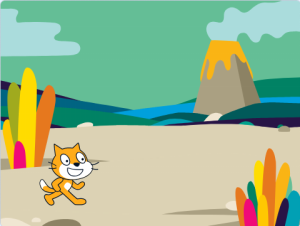
\includegraphics[width=.6\textwidth]{6.png}
        \end{minipage}
        \begin{minipage}{.68\textwidth}
            \begin{tasks}(2)
                \task 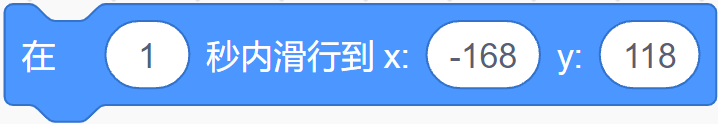
\includegraphics[width=.3\textwidth]{6a.png}
                \task 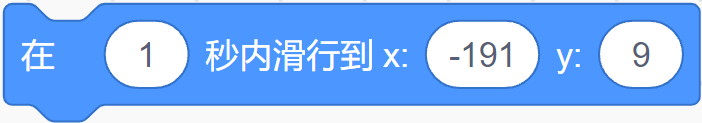
\includegraphics[width=.3\textwidth]{6b.png}
                \task 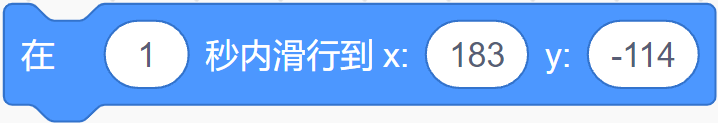
\includegraphics[width=.3\textwidth]{6c.png}
                \task 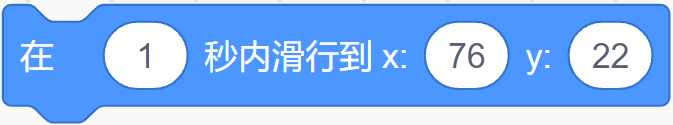
\includegraphics[width=.3\textwidth]{6d.png}
            \end{tasks}
        \end{minipage}

        % 7
        \item 有四只小老鼠一块出去偷食物(它们都偷食物了),回来时族长问它们都偷了什么食物.
        \begin{itemize}
            \item 老鼠A说:我们都偷了奶酪
            \item 老鼠B说:我只偷了一颗樱桃
            \item 老鼠C说:我没偷奶酪
            \item 老鼠D说:有些老鼠没偷奶酪
        \end{itemize}
        族长仔细观察了一下,发现它们当中只有一只老鼠说了真话.

        如果其中一只老鼠说的是真话,那么其他老鼠说的一定是假话,下面选项正确的是?(\qquad)
        \begin{tasks}(2)
            \task 所有老鼠都偷了奶酪
            \task 所有的老鼠都没有偷奶酪
            \task 有些老鼠没偷奶酪
            \task 老鼠B偷了一颗樱桃
        \end{tasks}

        \begin{figure}[htbp]
            \centering
            \begin{minipage}[t]{.23\textwidth}
                \centering
                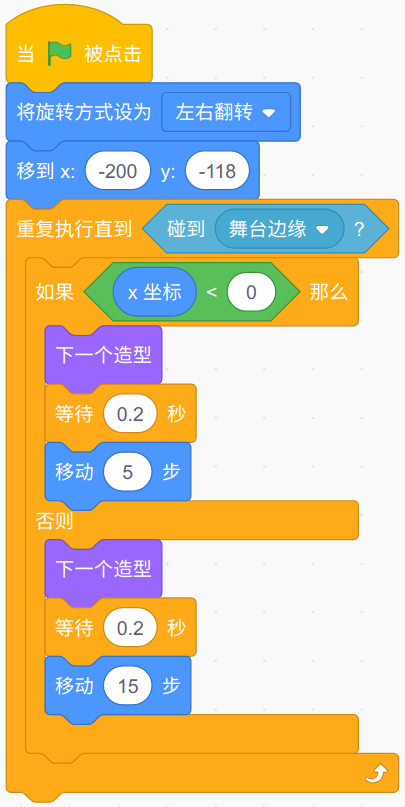
\includegraphics[width=.7\textwidth]{8.png}
                \caption*{第8题}
            \end{minipage}
            \begin{minipage}[t]{.23\textwidth}
                \centering
                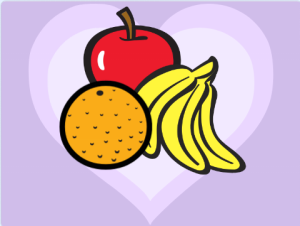
\includegraphics[width=.8\textwidth]{9.png}
                \caption*{第9题}
            \end{minipage}
            \begin{minipage}[t]{.23\textwidth}
                \centering
                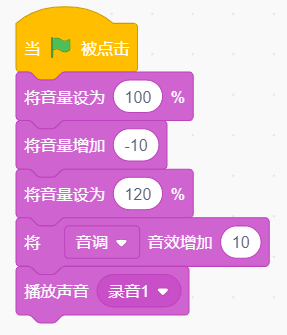
\includegraphics[width=.7\textwidth]{11.png}
                \caption*{第11题}
            \end{minipage}
        \end{figure}

       % 8
       \item 上面程序能够实现哪种跑步效果?(\qquad)
       \begin{tasks}(2)
           \task 小猫从左往右匀速跑步
           \task 小猫从右往左匀速跑步
           \task 小猫从左往右跑步,后半段加速跑
           \task 小猫从左往右跑步,后半段减速跑
       \end{tasks}

        % 9
        \item  三个水果的位置如上图所示,它们的层关系“从前到后”依次是?(\qquad)
        \begin{tasks}(4)
            \task 香蕉、苹果、橙子
            \task 橙子、香蕉、苹果
            \task 苹果、香蕉、橙子
            \task 橙子、苹果、香蕉
        \end{tasks}

        % 10
        \item 小明在编写控制机器人的程序时,为机器人录制自我介绍,使用下面哪个按钮,可以使得这段配音更符合机器人的特点、更加真实?(\qquad)
        \begin{center}
            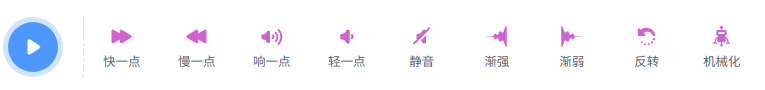
\includegraphics[width=.8\textwidth]{10.png}
        \end{center}
        \begin{tasks}(4)
            \task 响一点
            \task 机械化
            \task 慢一点
            \task 反转
        \end{tasks}

        % 11
        \item 执行如上图所示程序,角色的音量为?(\qquad)
        \begin{tasks}(4)
            \task 100
            \task 120
            \task 130
            \task 90
        \end{tasks}

        \newpage
        % 12
        \item 小猫初始位置在舞台中心,下面哪个选项可以实现小猫角色位置不停地随机变化?(\qquad)
        \begin{tasks}(4)
            \task 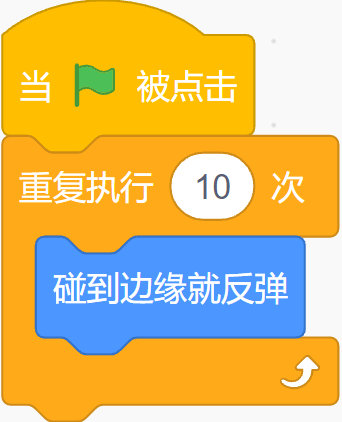
\includegraphics[width=.12\textwidth]{12a.png}
            \task 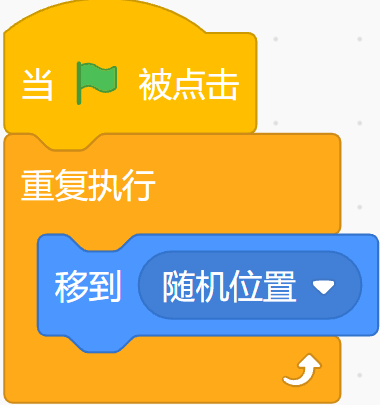
\includegraphics[width=.14\textwidth]{12b.png}
            \task 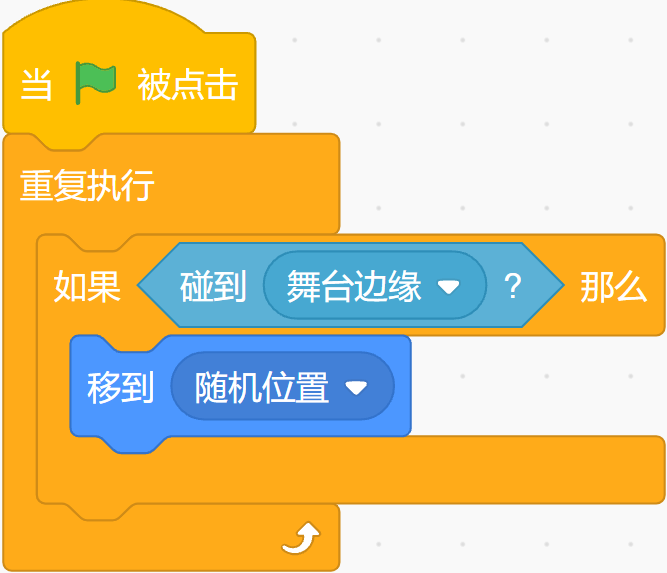
\includegraphics[width=.17\textwidth]{12c.png}
            \task 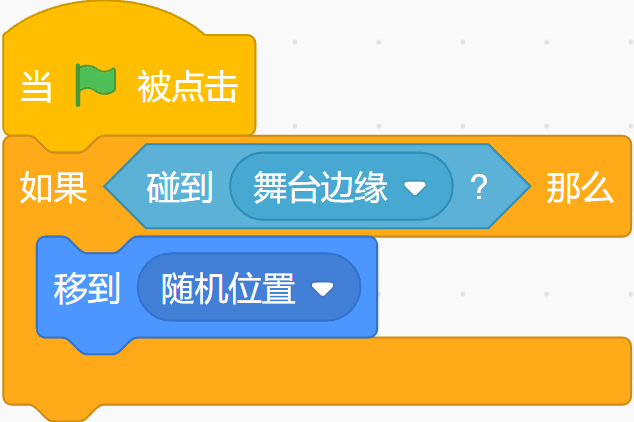
\includegraphics[width=.18\textwidth]{12d.png}
        \end{tasks}

        % 13
        \item 小明要编写一个循环15次的程序,使用下面哪个积木最容易实现?(\qquad)
        \begin{tasks}(4)
            \task 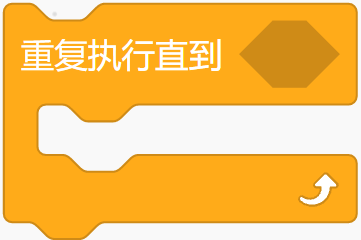
\includegraphics[width=.15\textwidth]{13a.png}
            \task 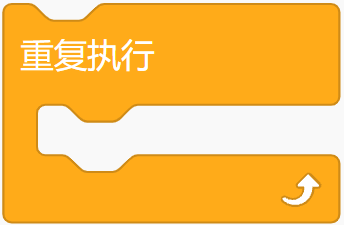
\includegraphics[width=.15\textwidth]{13b.png}
            \task 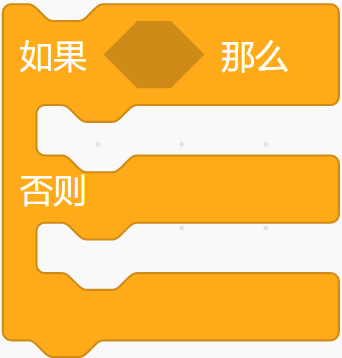
\includegraphics[width=.1\textwidth]{13c.png}
            \task 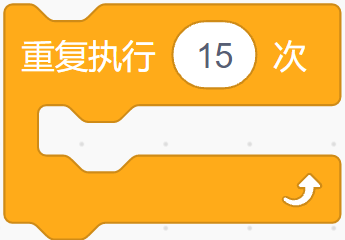
\includegraphics[width=.15\textwidth]{13d.png}
        \end{tasks}

        % 14
        \item 观察规律,丁处的图形应该是?(\qquad)
        \begin{tasks}(4)
            \task 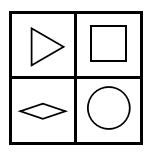
\includegraphics[width=.1\textwidth]{14a.png}
            \task 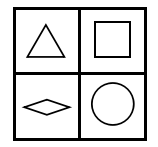
\includegraphics[width=.1\textwidth]{14b.png}
            \task 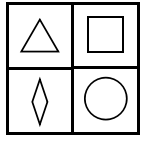
\includegraphics[width=.1\textwidth]{14c.png}
            \task 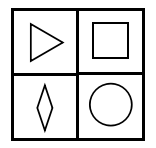
\includegraphics[width=.1\textwidth]{14d.png}
        \end{tasks}

        \begin{figure}[htbp]
            \centering
            \begin{minipage}[t]{.68\textwidth}
                \centering
                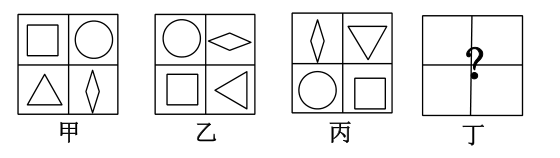
\includegraphics[width=0.7\textwidth]{14.png}
                \caption*{第14题}
            \end{minipage}
            \begin{minipage}[t]{.3\textwidth}
                \centering
                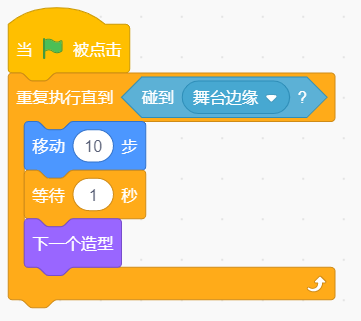
\includegraphics[width=.6\textwidth]{15.png}
                \caption*{第15题}
            \end{minipage}
        \end{figure}

        % 15
        \item  在“大鱼吃小鱼”游戏中,小鱼在海底世界随机位置出现后,不停地运动,并且在游动时切换造型,直到碰到舞台边缘停止移动。上图程序中什么语句让小鱼不停地运动?(\qquad)
        \begin{tasks}(4)
            \task 判断语句
            \task 循环语句
            \task 选择语句
            \task 顺序语句
        \end{tasks}

        % 16
        \item 小芳、小李、小强三人去买铅笔,有红、绿两种颜色可以选择,小李说选红色的,小芳说不选绿色的,小强和小李选的不一样,下面说法不正确的是?(\qquad)
        \begin{tasks}(2)
            \task 小强选的是绿色
            \task 有两个人选了红色
            \task 有两个人选了绿色
            \task 小芳和小李选的颜色一样
        \end{tasks}

        % 17
        \item  一件凶杀案,警察通过排查确定杀人凶手必为4个嫌疑犯的一个。以下为4个嫌疑犯的供词
        \begin{itemize}
            \item 1号说:不是我
            \item 2号说:是3号
            \item 3号说:是4号
            \item 4号说:3号在胡说
        \end{itemize}
        已知3个人说了真话,1个人说的是假话。根据以上这些信息,可以判断谁是凶手?(\qquad)
        \begin{tasks}(4)
            \task 1号
            \task 2号
            \task 3号
            \task 4号
        \end{tasks}

        % 18
        \item 只使用下面积木,不能编写循环结构程序的是?(\qquad)
        \begin{tasks}(4)
            \task 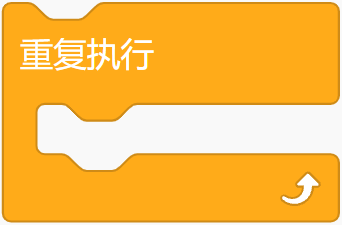
\includegraphics[width=.15\textwidth]{18a.png}
            \task 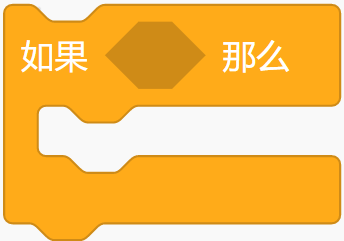
\includegraphics[width=.15\textwidth]{18b.png}
            \task 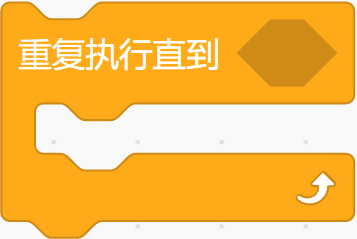
\includegraphics[width=.15\textwidth]{18c.png}
            \task 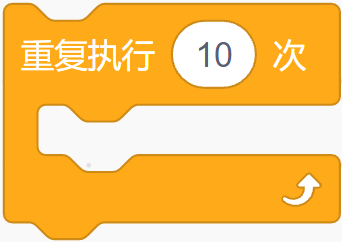
\includegraphics[width=.15\textwidth]{18d.png}
        \end{tasks}

        % 19
        \item  小猫程序和位置如下图所示,点击绿旗,小猫会说?(\qquad)
        \begin{tasks}(4)
            \task 我爱吃香蕉
            \task 我不爱吃香蕉
            \task 我爱吃苹果
            \task 我不爱吃苹果
        \end{tasks}

        \begin{figure}[htbp]
            \centering
            \begin{minipage}[t]{.5\textwidth}
                \centering
                \begin{minipage}[t]{.5\textwidth}
                    \centering
                    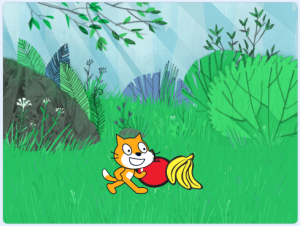
\includegraphics[width=\textwidth]{19-1.png}
                \end{minipage}
                \begin{minipage}[t]{.38\textwidth}
                    \centering
                    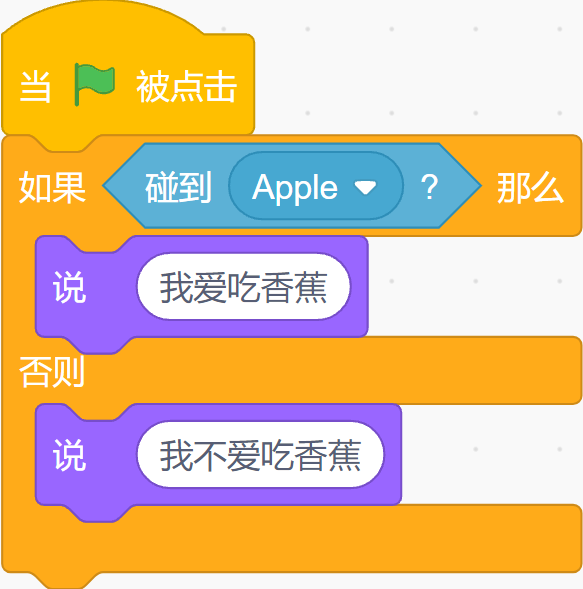
\includegraphics[width=\textwidth]{19-2.png}
                \end{minipage}
                \caption*{第19题}
            \end{minipage}
            \begin{minipage}[t]{.25\textwidth}
                \centering
                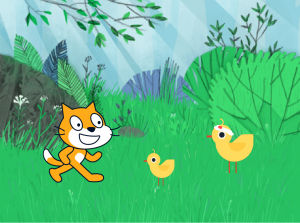
\includegraphics[width=\textwidth]{20.png}
                \caption*{第20题}
            \end{minipage}
            \begin{minipage}[t]{.14\textwidth}
                \centering
                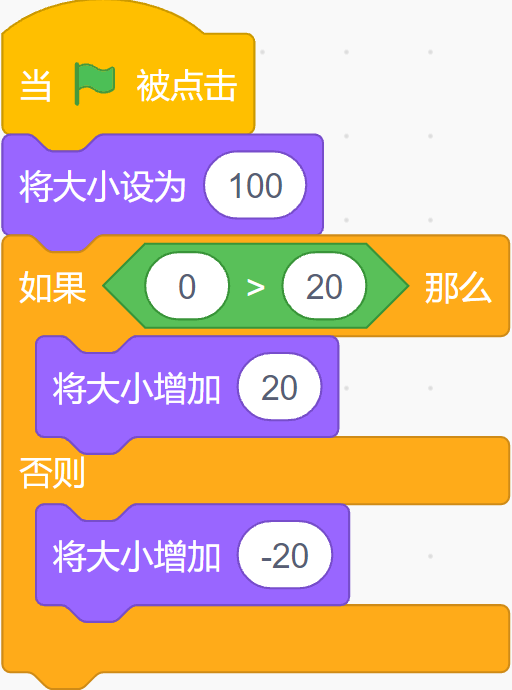
\includegraphics[width=\textwidth]{23.png}
                \caption*{第23题}
            \end{minipage}
        \end{figure}

        % 20
        \item  如上图所示,小猫在森林中散步,看到了小鸡和受伤的鸡妈妈,使用下面哪个积木可以让小猫碰到鸡妈妈后,带鸡妈妈去医院?(\qquad)
        \begin{tasks}(2)
            \task 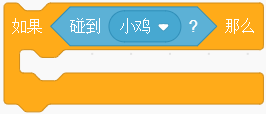
\includegraphics[width=.18\textwidth]{20a.png}
            \task 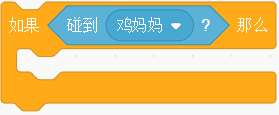
\includegraphics[width=.18\textwidth]{20b.png}
            \task 都不对
            \task 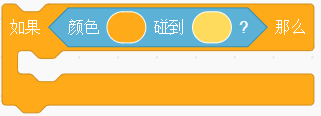
\includegraphics[width=.18\textwidth]{20d.png}
        \end{tasks}

        % 21
        \item 小明非常喜欢画画,下面哪个积木可以擦除画笔画出的痕迹?(\qquad)
        \begin{tasks}(4)
            \task 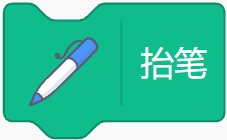
\includegraphics[width=.1\textwidth]{21a.png}
            \task 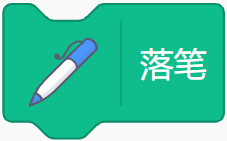
\includegraphics[width=.1\textwidth]{21b.png}
            \task \includegraphics[width=.13\textwidth]{21c.png}
            \task \includegraphics[width=.1\textwidth]{21d.png}
        \end{tasks}

        % 22
        \item 小明做了一个寻宝游戏,输入密码后,使用下面哪个积木能实现密码正确则宝箱会被打开,反之则显示“密码错误”?(\qquad)
        \begin{tasks}(4)
            \task \includegraphics[width=.15\textwidth]{22a.png}
            \task \includegraphics[width=.15\textwidth]{22b.png}
            \task \includegraphics[width=.1\textwidth]{22c.png}
            \task \includegraphics[width=.15\textwidth]{22d.png}
        \end{tasks}

        % 23
        \item  执行上图代码后,小猫的大小是多少?(\qquad)
        \begin{tasks}(4)
            \task 0
            \task 80
            \task 100
            \task 120
        \end{tasks}

        \newpage
        % 24
        \item 按下键盘上的哪个键,苹果将出现在下图位置?(\qquad)
        \begin{tasks}(4)
            \task a
            \task b
            \task c
            \task d
        \end{tasks}

        \begin{figure}[htbp]
            \centering
            \begin{minipage}[t]{.45\textwidth}
                \centering
                \begin{minipage}[t]{.42\textwidth}
                    \centering
                    \includegraphics[width=\textwidth]{24-1.png}
                \end{minipage}
                \begin{minipage}[t]{.55\textwidth}
                    \centering
                    \includegraphics[width=\textwidth]{24-2.png}
                \end{minipage}
                \caption*{第24题}
            \end{minipage}
            \begin{minipage}[t]{.25\textwidth}
                \centering
                \includegraphics[width=\textwidth]{26.png}
                \caption*{第26题}
            \end{minipage}
            \begin{minipage}[t]{.25\textwidth}
                \centering
                \includegraphics[width=\textwidth]{27.png}
                \caption*{第27题}
            \end{minipage}
        \end{figure}

        % 25
        \item 下面哪个选项的结果是3?(\qquad)
        \begin{tasks}(4)
            \task \includegraphics[width=.15\textwidth]{25a.png}
            \task \includegraphics[width=.15\textwidth]{25b.png}
            \task \includegraphics[width=.1\textwidth]{25c.png}
            \task \includegraphics[width=.15\textwidth]{25d.png}
        \end{tasks}
    \end{enumerate}

    % 判断题
    {\noindent\textbf{第二部分、判断题(共 10 题,每题 2 分,共20分.)}}
    \begin{enumerate}
        \setcounter{enumi}{25}
        % 26
        \item 上面两个程序,执行的结果是一样的.(\qquad)

        %27
        \item 判断按下“a”键,可以使用上面积木.(\qquad)

        %28
        \item  积木\includegraphics[width=.2\textwidth]{28.png}的运行的结果是19.(\qquad)
  
        %29
        \item 有甲、乙两同学,其中一个人有奇数根铅笔,一个人有偶数根铅笔。如果再给甲原有的铅笔数,再给乙原有铅笔数的2倍,他们俩共有铅笔数为偶数。那么,甲同学原有铅笔数是偶数.(\qquad)
        
        %30
        \item 执行以下两组积木是完全一样的,都需要判断两次条件是否成立.(\qquad)
        
        %31
        \item 下面积木的功能是: 如果条件成立,那么执行该积木中的第一个分支;如果条件不成立,那么就执行积木中的第二个分支.(\qquad)
        
        \begin{figure}[htbp]
            \centering
            \begin{minipage}[t]{.18\textwidth}
                \centering
                \includegraphics[width=.7\textwidth]{31.png}
                \caption*{第31题}
            \end{minipage}
            \begin{minipage}[t]{.18\textwidth}
                \centering
                \includegraphics[width=\textwidth]{32.png}
                \caption*{第32题}
            \end{minipage}
            \begin{minipage}[t]{.33\textwidth}
                \centering
                \includegraphics[width=\textwidth]{35.png}
                \caption*{第35题}
            \end{minipage}
        \end{figure}
        
        %32
        \item 上面积木,条件成立时,循环结束,执行这个积木后面的程序.(\qquad)
                
        %33
        \item Scratch可以对声音进行简单的剪辑.(\qquad)
        
        %34
        \item  小明非常喜欢画画,他想当一名画家,在绘画开始之前,可以使用\includegraphics[width=.2\textwidth]{34.png}积木设置画笔的颜色为绿色.(\qquad)
        
        %35
        \item 上面两个程序运行的效果是一样的.(\qquad)
    \end{enumerate}

    \newpage
    {\noindent \textbf{第三部分、编程题(共 2 题,共30分.)}}
    \begin{enumerate}
        \setcounter{enumi}{35}
        
        % 36
        \item 寻找宝石:
        \begin{figure}[htbp]
            \begin{minipage}{.6\textwidth}
                1. 准备工作
                \begin{tasks}[label = (\arabic*)]
                    \task 背景:Blue Sky2;
                    \task 角色:Cat、Crystal、回形迷宫(手绘).
                \end{tasks}
                2. 功能实现
                \begin{tasks}[label = (\arabic*)]
                    \task 如左图所示,将小猫和宝石放置在迷宫左下角位置,中间有白墙分隔,调整小猫和宝石的大小;
                    \task 利用键盘的上下左右键分别控制小猫面向四个方向移动,移动过程中小猫脑袋不朝下;
                    \task 小猫在移动的过程中不能碰到白墙,否则返回原点;
                    \task 当小猫成功碰到宝石,说“游戏胜利”,全部程序停止.
                \end{tasks}
            \end{minipage}
            \begin{minipage}{.37\textwidth}
                \centering
                \includegraphics[width=\textwidth]{36.png}
            \end{minipage}
        \end{figure}

        %37
        \item 两座对称的山峰:
        \begin{figure}[htbp]
            \begin{minipage}{.6\textwidth}
                1. 准备工作
                \begin{tasks}[label = (\arabic*)]
                    \task 背景:Xy-grid;
                    \task 角色:任意.
                \end{tasks}
                2. 功能实现
                \begin{tasks}[label = (\arabic*)]
                    \task 隐藏添加的角色;
                    \task 调整画笔颜色为“黑色”,粗细为“5”;
                    \task 当按下键盘的“L”键,画出左侧三角形;
                    \task 当按下键盘的“R”键,画出右侧三角形;
                    \task 落在$x$轴的三个顶点分别为$(-100,0)$、$(0,0)$、$(100,0)$;
                    \task 以$y$轴为对称轴,左右对称.
                \end{tasks}
            \end{minipage}
            \begin{minipage}{.37\textwidth}
                \centering
                \includegraphics[width=\textwidth]{37.png}
            \end{minipage}
        \end{figure}
    \end{enumerate}
\end{document}